\DiaryEntry{Order Statistics, 2}{2018-01-10}{Stochastic}

Consider $N=3$ RVs each with uniform distribution. The distribution of minimum and maximum has been done (part 1), this entry deals with the statistics of $X_{(2)}$. Using the previous results, we obtain for $N=3, k=2$,

\bee
F_2(x) = \sum_{i=2}^3 {3 \choose i} F^i(x) \left[ 1 - F(x) \right]^{3-i}
\eee

which can be expanded into

\bee
F_2(x) = 3 F^2(x) \left[ 1 - F(x) \right] + F^3(x)
\eee

With the cdf of the uniform distribution

\bee
F(x) = \begin{cases}
	0 \quad &x < 0 \\
	x \quad &0 \geq x \geq 1 \\
	1 \quad &x > 1
\end{cases}
\eee

we obtain

\bee
F_1(x) = \begin{cases}
	0 \quad &x < 0 \\
	3x^2(1-x) + x^3 = x^2(3-2x)\quad &0 \geq x \geq 1 \\
	1 \quad &x > 1
\end{cases}
\eee

The corresponding pdf is

\bee
f_1(x) = \begin{cases}
	0 \quad &x < 0 \\
	6x(1-x) \quad &0 \geq x \geq 1 \\
	1 \quad &x > 1
\end{cases}
\eee 

The following plot shows the estimated pdf (y2) compared to the analytical result (y1). It is somewhat intuitive that the "mid-value" $X_{(2)}$ is most likely to be around $1/2$.

\begin{figure}[H]
	\centering
	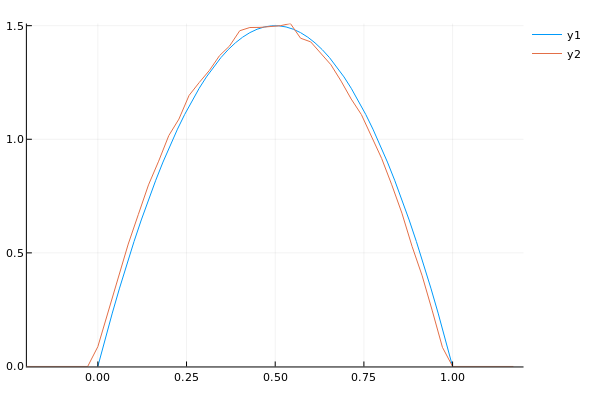
\includegraphics[scale=0.7]{images/order_stat_2_1.png}
\end{figure}

For increasing values of odd $N$, the distribution of the "mid-value" $X_{((N+1)/2)}$ is symmetric around $1/2$ and becomes more and more peaky. This can be explained by the fact that more and more RVs are placed into the fixed interval $[0,1]$ and therefore the mid-value becomes more peaky.
